\section{Radio Controller}
The radio controller, used to steer the boat, is a Radiolink AT9 9 channel 2.4GHz control system. The controller supports the provided Radiolink R9D receiver which is a 9 channel, 2.4 GHz DSSS (Direct-sequence spread spectrum) receiver.
\subsection{Steering}
The Layout of the buttons on the controller can be seen in Figure \ref{fig:controller_front}, and \ref{fig:controller_back} for the front, and back of the controller respectively. In Figure \ref{fig:controller_front} the \textit{Rudder/Elevator stick} is used to control the speed of propellers driving the boat forward. The propellers will be still when the stick is in the lowest position in the figure, and will have max speed when the stick is in the top most position in the figure. Note that the stick should be put in the lowest position when the electronics of the boat is powered on.

The \textit{Throttle/Aileron Stick} is used to control the air rudder. Moving the stick to the right will turn the boat to the right and moving it to the left will turn the boat left.

The stick on the back of the controller, the \textit{VRC SW} stick in Figure \ref{fig:controller_back} is used to control the rotational speed of the RBRs. If the stick is in the bottom most position the RBRs will not rotate. By moving the stick upwards the speed will increase until the stick is in the top position.


% Latexkod för bilderna jag lagt i denna mapp
\begin{figure}[p]
   \centering
   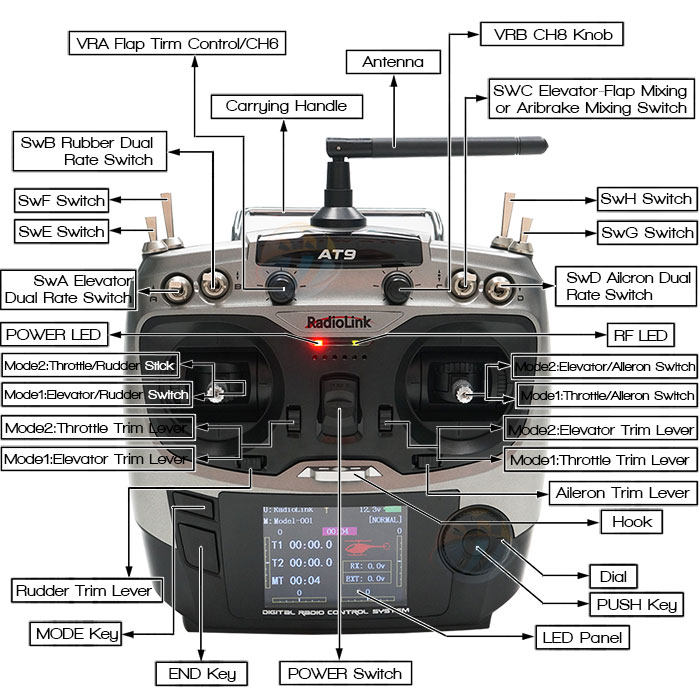
\includegraphics[width=.75\textwidth]{controller_front}
   \caption{The front of the radio controller and its buttons.}
   \label{fig:controller_front}
\end{figure}

\begin{figure}[p]
   \centering
   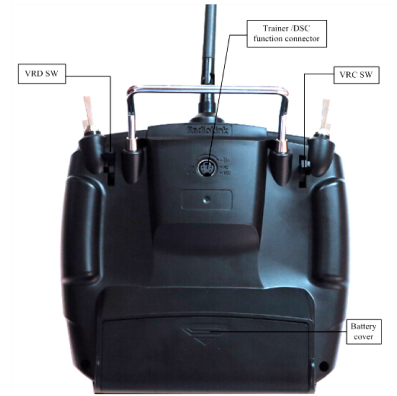
\includegraphics[width=.75\textwidth]{controller_back}
   \caption{The back of the radio controller and its buttons.}
   \label{fig:controller_back}
\end{figure}

\subsection{Settings}
When it comes to the settings in the controlled we used the base settings of the Helicopter type, which can be found under \textit{Model sel.} in the basic menu of the controller. The basic menu is found by holding in the \textit{mode} button. Some settings however were changed to be able to maneuver the vehicle more easily. The first of these setting tweaks were to put channel 1-3 from normal to reversed, in order to get the buttons to behave in a way better suited for a boat. This is done in \textit{reverse}, which can be found in the Basic menu. In order to get the \textit{VrC SW} button on the back of the controller, used to control the rotational speed of the RBRs (see Figure \ref{fig:controller_back} for button layout), one has to go into \textit{AUX-CH} in the basic menu and choose which channel  one want to couple it with. Then select \textit{VrC} on that channel. We chose to use channel 5 but any other channel can be used as well.
